\section{Origin of torque ripple}

%Ripples due to mechanical parts cannot be estimated from the electrical subsystem \cite{ILC:2018}. All possible sources of torque ripples are observable from the rotor speed \cite{ILC:2018}. 
In this chapter, all important factors affecting torque ripple are discussed. FEA is utilized for analyzing torque ripple and its sources. A model of a 160-kW motor is used and its parameters are listed in Table \ref{FEM_motor_params}. The motor cross section in Fig. \ref{FEM_flux} shows the magnet placement, stator slots as well as flux density distribution of the PM motor.

\begin{table}[ht]
\caption{160-kW PM motor parameters}
\centering
\begin{tabular}[t]{lcccc}
\hline
Description       & Symbol     & Value  & Unit\\
\hline
Nominal current   & $I_N$      & 332.1  & A\\
Nominal voltage   & $U_N$      & 370.0  & V\\
Nominal frequency & $f_N$      & 155.0  & Hz\\
Nominal speed     & $\omega_N$ & 3100   & rpm\\
Nominal power     & $P_N$      & 160.0  & kW\\
Nominal torque    & $T_N$      & 493.0  & Nm\\
Number of poles   & $N_p$      & 6     & \\
Number of stator slots & $N_s$ & 72     & \\
\hline
\label{FEM_motor_params}
\end{tabular}
\end{table}%

\begin{figure}[htb] 
    \centering
    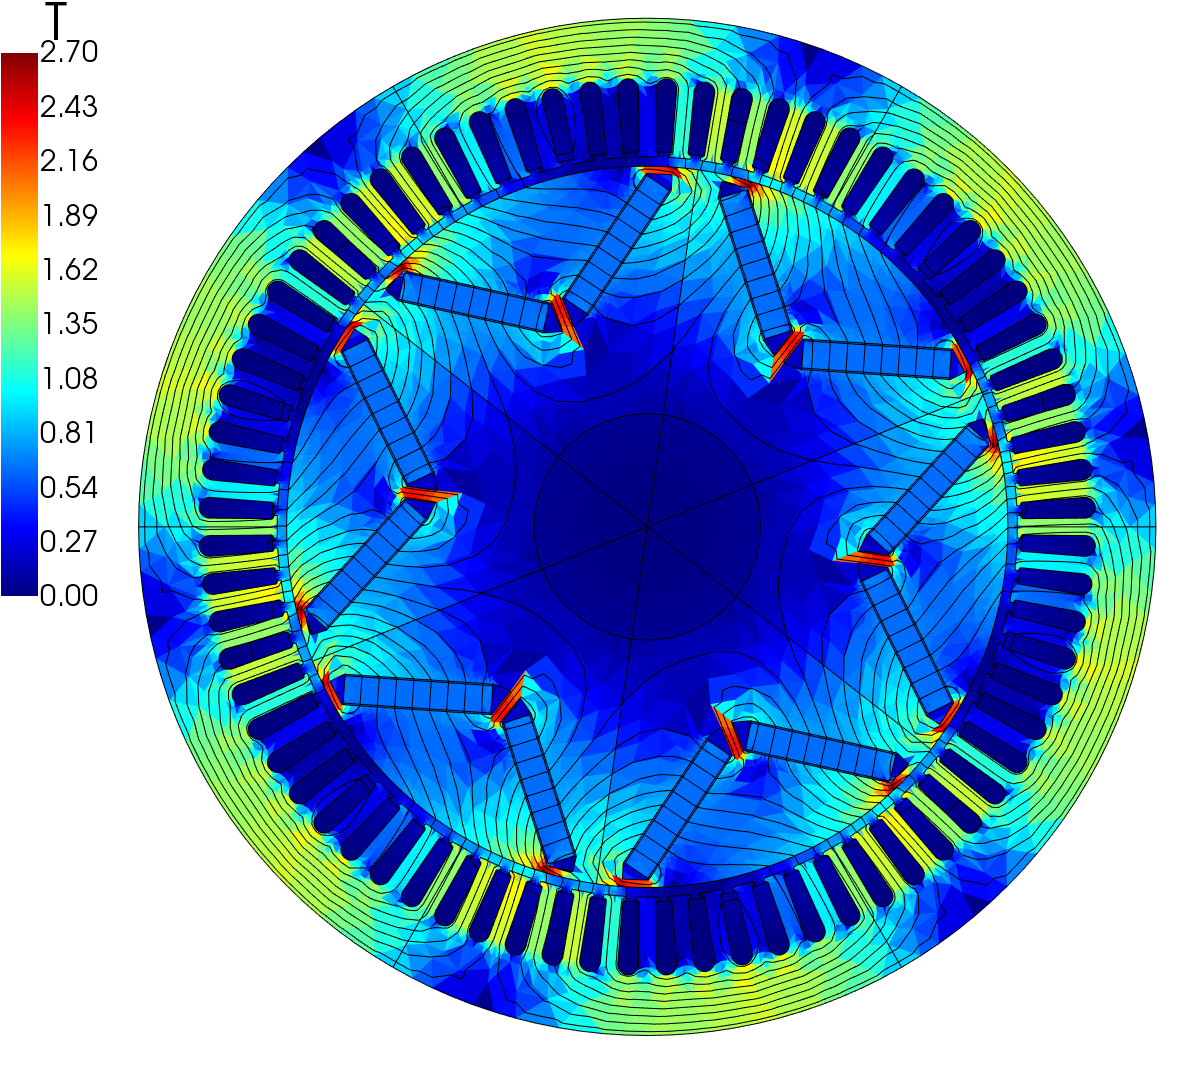
\includegraphics[width=0.6\linewidth]{images/flux_density.png} 
    \caption{Flux density distribution of the $160$-kW PM motor at the nominal point} 
    \label{FEM_flux} 
\end{figure}

\subsection{PMSM model} \label{PMSM model}

Assuming that eddy currents and hysteresis losses are negligible, stator surface is smooth and magnetomotive force (MMF) of the stator windings is sinusoidal, the flux linkages along the d–q axes in the rotor reference frame are given by \cite{Vector-control} % check citation
\begin{equation}
    \begin{split}
        & \psi_{d} = L_{d} i_{d} + \psi_f
        \\[2ex]
        & \psi_{q} = L_{q} i_{q}
    \end{split}
    \label{Eq:flux-linkages}
\end{equation}
where $i_d$ and $i_q$ are the dq-axis currents, $L_d$ and $L_q$ are dq-axis inductances and $\psi_f$ is the rotor flux linkage. By further assuming the PMSM to be nonsalient, the $L_d$ and $L_q$ can be considered equal \cite{ILC:2005}. Stator dq-axis voltages can be expressed as \cite{Vector-control}
\begin{equation}
    \begin{split}
        & u_{d} = R_s i_{d} + \frac{d \psi_{d}}{dt} - \omega_e \psi_{q} 
        \\[2ex]
        & u_{q} = R_s i_{q} + \frac{d \psi_{q}}{dt} + \omega_e \psi_{d}
    \end{split}
     \label{Eq:voltage}
\end{equation}
where $\omega_e$ is the electrical angular speed of the rotor and $R_s$ is the stator resistance.

Electromagnetic torque can be expressed as \cite{Vector-control, ILC:2012, ILC:2018}
\begin{equation}
    T_m = \frac{3}{2}p(\psi_{d} i_{q} - \psi_{q} i_{d})
    \label{torque_eq}
\end{equation}
where $p = N_p/2$ is the number of pole pairs. With field-oriented control, the d-axis current is controlled to be zero in order to maximize the output torque with given current \cite{ILC:2012, Vector-control}. Hence, only q-axis current is used for torque production and with $i_{d} = 0$, the torque equation reduces to
\begin{equation}
    T_m = \frac{3}{2}p \psi_f i_{q} = k_t i_{q}
    \label{torque_eq2}
\end{equation}
where $k_t$ is a torque coefficient.

In order to make the model to reflect non-ideal reality more accurately, also possible disturbances should be considered. Therefore, coefficients describing cogging torque and current measurement errors are added to the electromagnetic torque equation \cite{ILC:2004}
\begin{equation}
    T_m = k_t i_{q} + T_{cog} + T_{\Delta I}
    \label{torque_eq3}
\end{equation}
where $T_{cog}$ and $T_{\Delta I}$ are periodic torque pulsations due to cogging torque and current measurement errors, respectively.
% Mention that high speeds the pulsation effect is not as strong -- dampening. use inertai eq.

The equation of motion is
\begin{equation}
    \frac{d \omega_m}{dt} = -\frac{B}{J}\omega_m + \frac{T_m}{J} - \frac{T_l}{J}
    \label{PMSM_dynamics}
\end{equation}
where $\omega_m = \omega_e / p$ is the mechanical angular speed, $T_l$ is the load torque, $B$ is the viscous damping coefficient and $J$ is the total inertia (motor and load) \cite{ILC:2005}. 
%From this equation, it can be concluded that speed fluctuations decrease when the inertia increases.

\subsection{Relation between torque and speed pulsations}

%Higher rotation speeds can be seen to increase the inertia which in turn leads to reduced fluctuations. Speed increase shifts the torque ripple to a higher frequency and therefore its negative effects to speed weaken. Due to spontaneous dampening, the active ripple minimization is not as important at high speeds as it is on low speeds.

%Increase in the speed shifts the torque ripple to a higher frequency.
The 160-kW motor was run with a constant speed reference in a simulation environment. The FEM simulation was repeatedly stepped forward while instantaneous torque and rotor speed were numerically computed. Motion equation \eqref{PMSM_dynamics} was used in the simulation. Computation result in Fig. \ref{SDM_speed_torque} shows undesired speed and torque fluctuations, even when the machine speed was controlled with a PI controller and the speed reference was kept constant. Thereby, disturbances must be present, since the system never stabilizes.
\begin{figure}[htb]
    \centering
    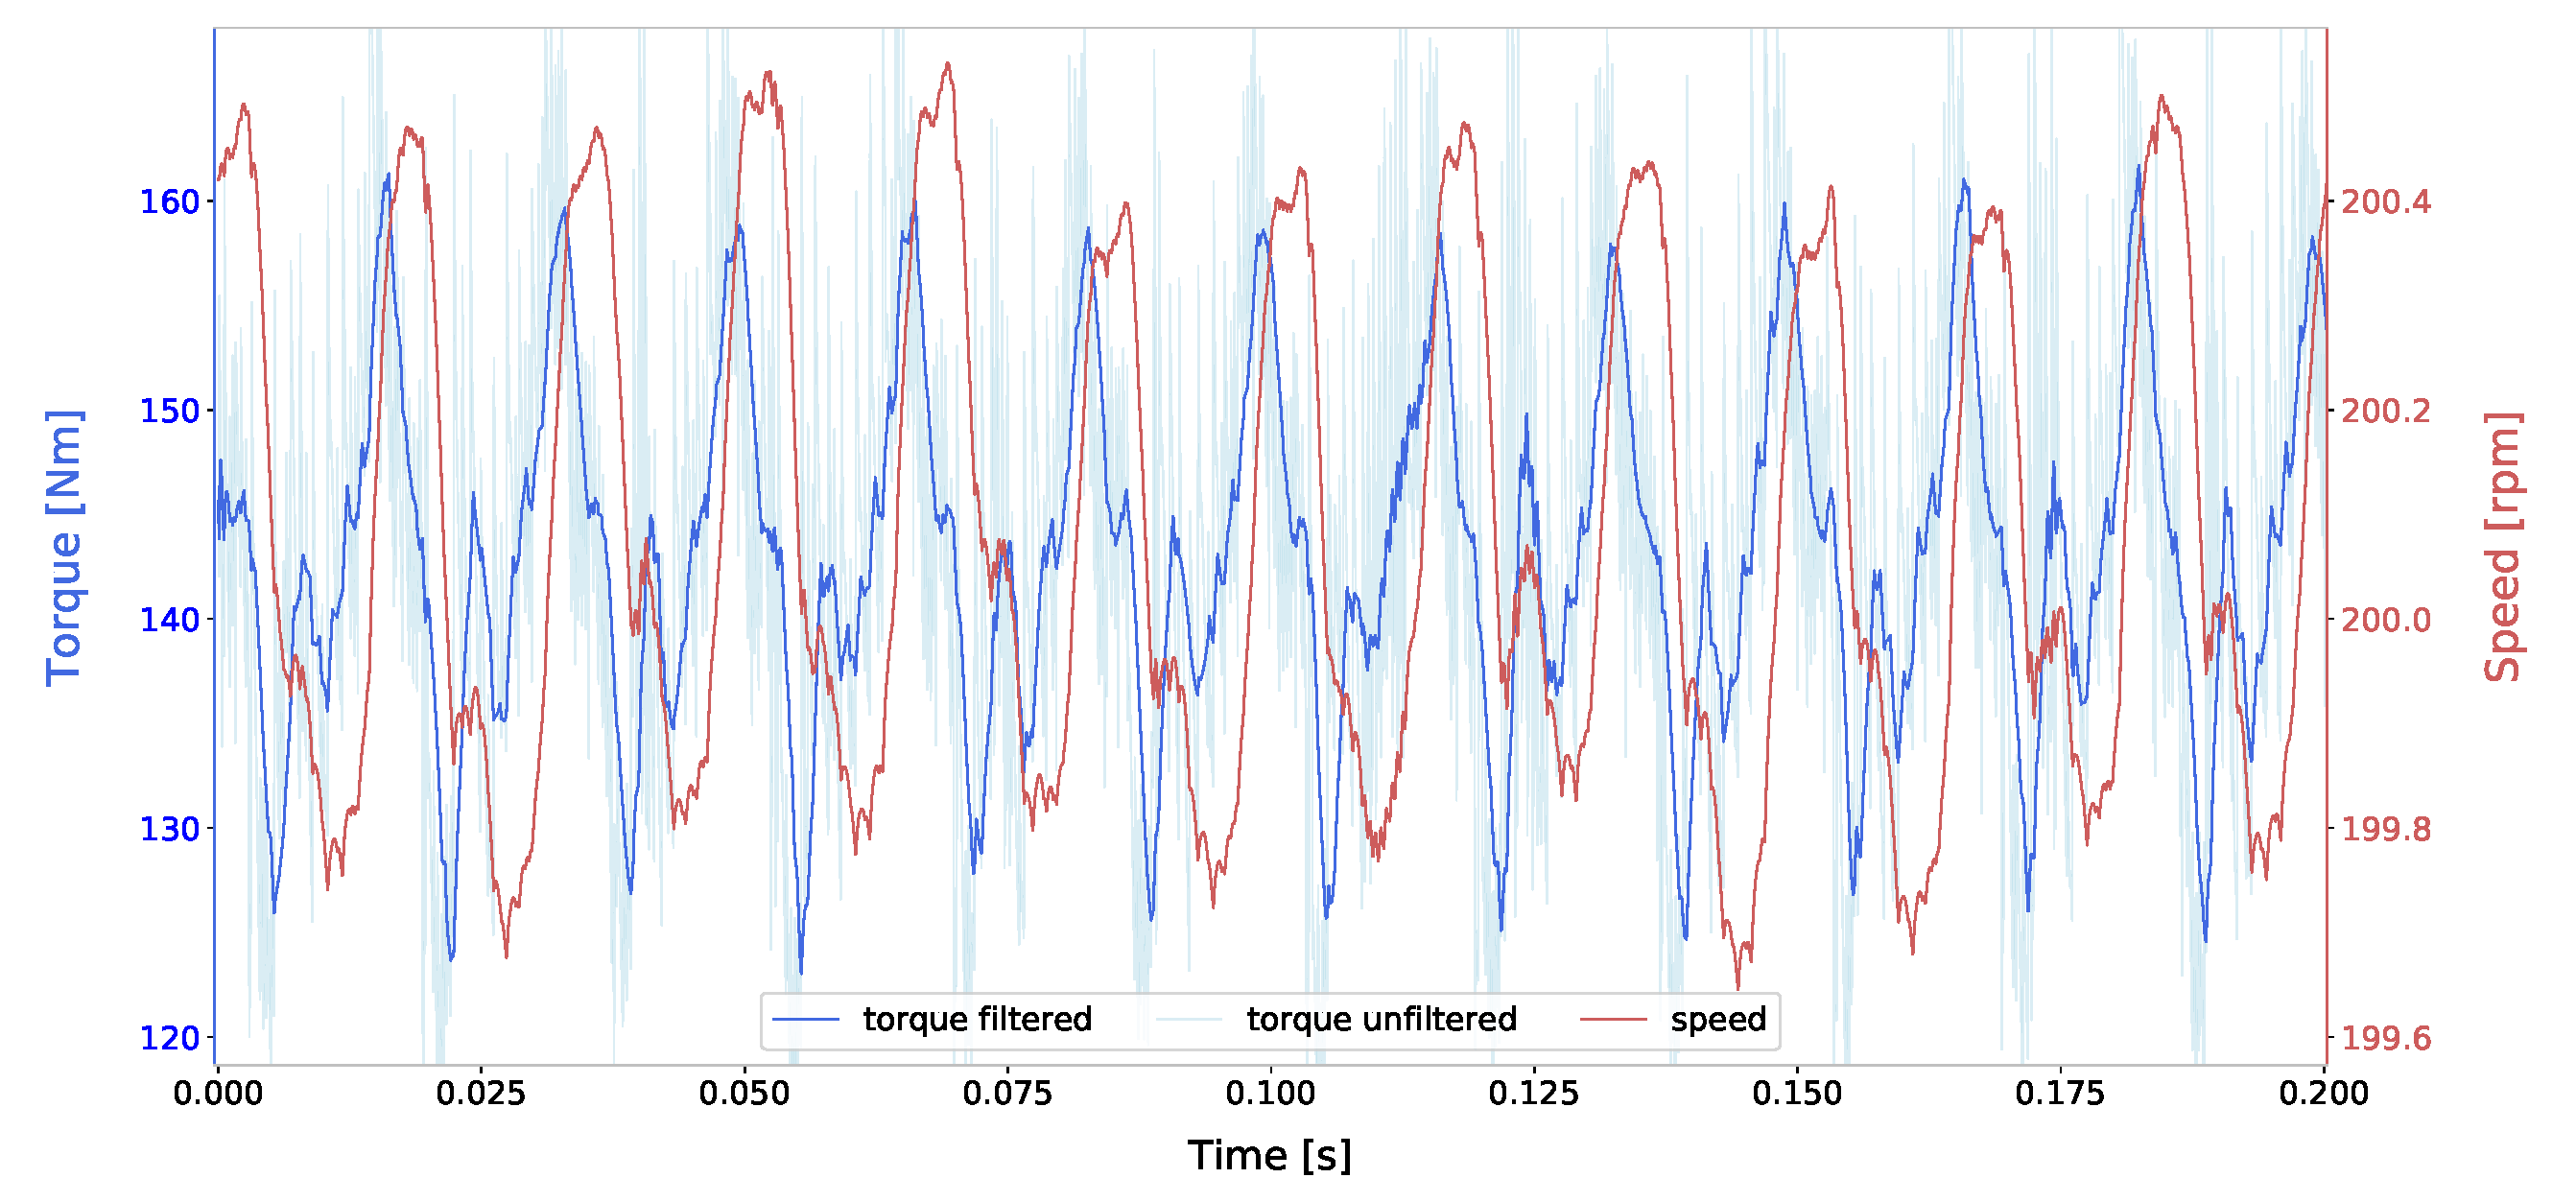
\includegraphics[width=1\linewidth]{images/torque-speed-pulsations.pdf}
    \caption{Torque and speed pulsations of the 160-kW motor}
    \label{SDM_speed_torque} 
\end{figure}

%\begin{figure}[htb] 
%    \centering
%    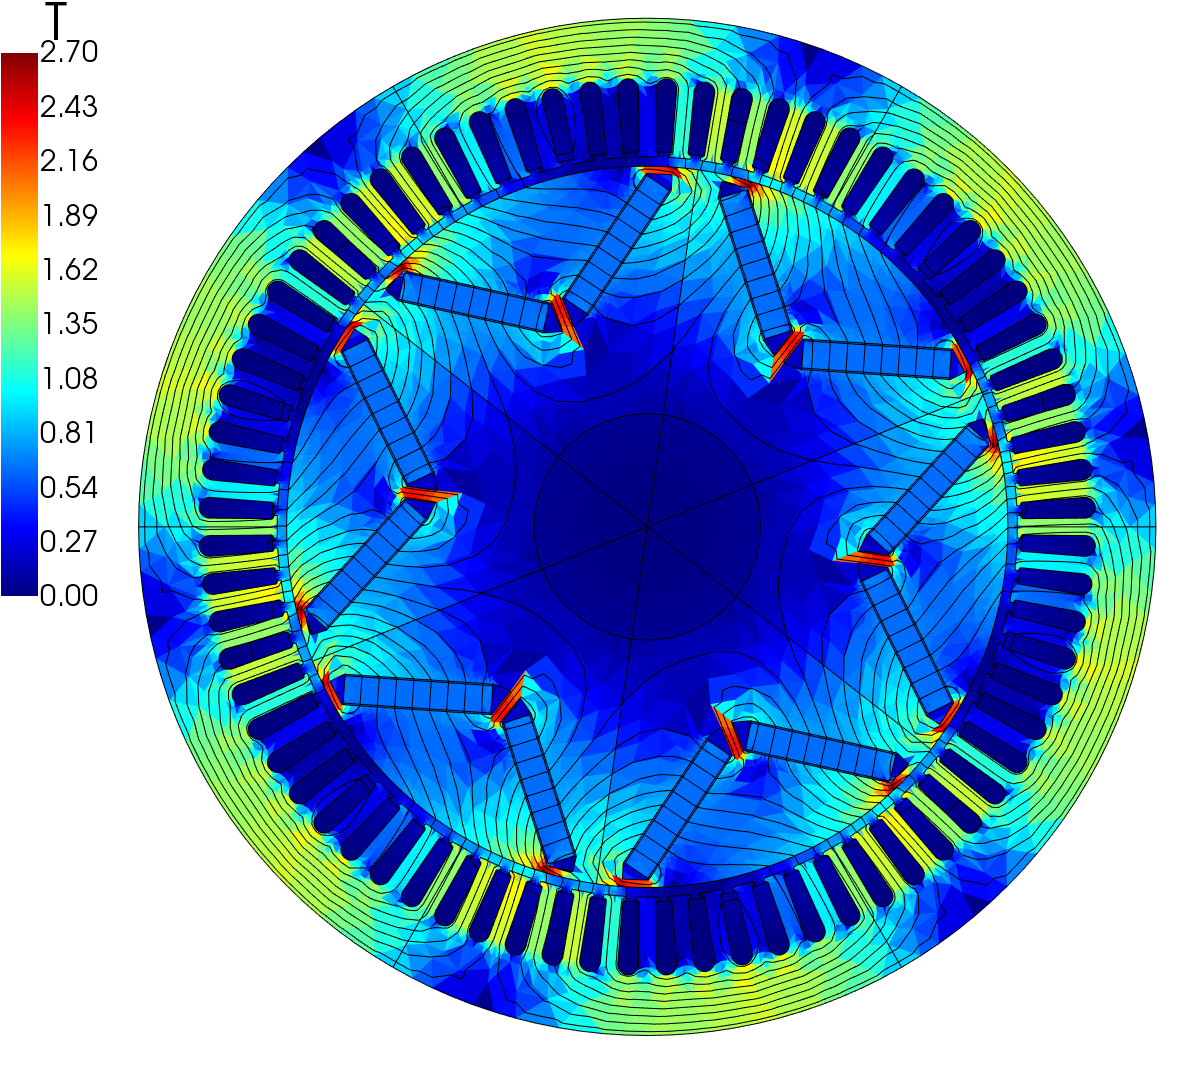
\includegraphics[width=0.6\linewidth]{images/flux_density.png} 
%    \caption{Flux density distribution of the $160$-kW PM motor} 
%    \label{FEM_flux} 
%\end{figure}

% With higher frequencies, the speed oscillations diminish spontaneously.
%With higher frequencies, the speed oscillations diminish spontaneously. This can be reasoned from the frequency response corresponding to \eqref{Eq:transfer_function}.

Equation \eqref{PMSM_dynamics} allows to derive the transfer function between mechanical angular velocity $\omega_m$ and electromagnetic torque $T_m$
\begin{equation}
    \omega_m(s) = \frac{T_m(s) - T_l(s)}{Js + B}
    \label{Eq:transfer_function}
\end{equation}
It can be concluded that speed oscillates at the same harmonic frequencies as electromagnetic torque \cite{ILC:2005, ILC:2018}. The same can be also observed from Fig. \ref{SDM_speed_torque} by comparing speed and torque oscillations. The relation between pulsations makes it possible to measure speed signal in order to indirectly conclude whether torque pulsations exist \cite{ILC:2005}. To minimize the speed pulsations, its source, torque pulsations, must be minimized \cite{ILC:2004, ILC:2018}. This relation makes it possible to utilize speed measuring instruments, such as resolvers and encoders in ripple minimization. When ripple minimization method is based on speed measurements, the compensator becomes more widely applicable, because encoders and resolvers are more commonly available than torque transducers.

Another FEM computation was performed at different speeds and in open-circuit condition. The result is visualized in Fig. \ref{FEM_orders}. Harmonic orders are given with respect to the mechanical frequency of the rotor. It can be observed that torque amplitudes are equal regardless of the speed. Therefore, the rotation speed is irrelevant when studying harmonics and data can be visualized in two dimensional space without losing information.
\begin{figure}[htb] 
    \centering
    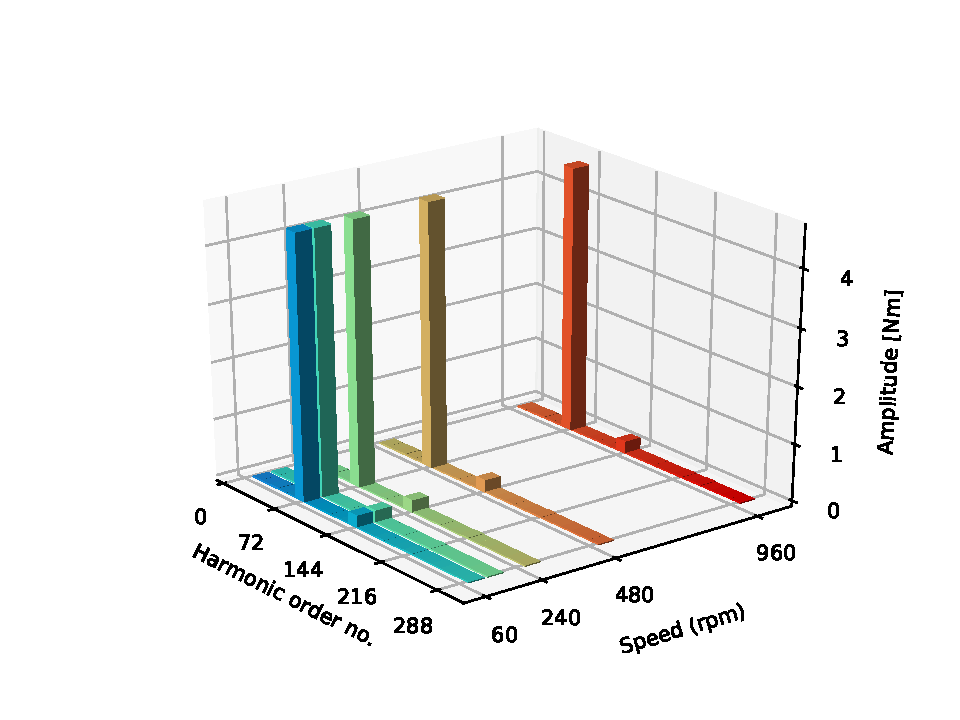
\includegraphics[width=1.0\linewidth]{images/cogging-different-speeds.pdf} 
    \caption{Cogging torque of the 160-kW motor in different speeds}
    \label{FEM_orders}
\end{figure}
%in which the harmonic orders are given with respect to the mechanical frequency of the rotor, 
% Harmonic order into picture and to text:
% Harmonic order considering the mechanical frequency of the rotor as the fundamental frequency
% considering the mechanical frequency of the rotor as the fundamental frequency

%Torque data was computed with respect to the rotor angle and then the amplitudes of certain harmonic orders were collected. Thereby, Fig. \ref{FEM_orders} shows cogging torque of the 160-kW motor in different operating points. Since sampling was done with respect to the rotor angle, the sampling frequency had to be altered between different computations. When speed was doubled, the sampling frequency had to be halved in order to maintain a constant sampling rate. This practice would eventually lead to aliasing, thus only a few operating points were captured and the initial sampling rate was set very high.

% ===================================================================================================================
\subsection{Cogging torque}

% Application of a multiobjective.. \cite{TRR:1999}
% Comparison of Cogging.. \cite{CTR_HW:2013}
% simulation:2011

Cogging torque arises from interaction between magnets and stator teeth. The magnets create magnetic field around the rotor whilst slots in stator induce permeance variation in airgap. Due to permeance variation, the rotor seeks a position where the permeance of the magnetic circuit is maximized \cite{TRR:1999, CTR_HW:2013}. This creates periodic torque on the shaft, which may generate undesired mechanical vibrations and noise. Since torque pulsations give rise to speed oscillations similarly to Fig. \ref{SDM_speed_torque}, also accurate position control gets more difficult. This explains why ripple minimization is particularly important with servomotors. 

%The pulsations and their relation can be seen from Fig. \ref{SDM_speed_torque}, which shows measured speed and estimated torque of a loadless PM servomotor. Due to inertia (see Eq. \ref{PMSM_dynamics}), the speed varies more moderately than the torque estimate. Additionally, a small delay between the signals can be observed. The gains of the speed controller were set low to produce smooth signal.

%The pulsations in Fig. \ref{SDM_speed_torque} are generated mostly by cogging torque, since the speed reference was kept constant $60$ rpm and no load was connected to the shaft of the servomotor.

%\begin{figure}[ht]
%    \centering
%    \includegraphics[width=1\linewidth]{images/torque_speed_pulsations.pdf}
%    \caption{Torque and speed pulsations of a PM servomotor (SDM-251)}
%    \label{SDM_speed_torque} 
%\end{figure}

Cogging torque can be expressed as Fourier series \cite{CTR_HW:2002, CTR_HW:2004, cogging:2006, CTR:2010, CTR_HW:2013, CTR_HW_skew:2013, CTR_SW:2017, CTR_HW:2017}. For a single slot, the cogging torque is given by \cite{cogging:2006, CTR_HW:2013}
\begin{equation}
    T_{cslot}(\theta_m) = \sum_{i=\text{1,2,3,...}}^{\infty} A_i \, \sin(N_pi\theta_m)
    \label{eq_cogging_torque1}
\end{equation}
where $N_p$ is the number of poles, $\theta_m$ gives the rotor position relative to single stator slot and $A_i$ is the amplitude of the corresponding $i$th harmonic. Since $\theta_e = (N_p/2)\theta_m$, harmonics can be also considered as a function of the electrical rotor angle, $\theta_e$ \cite{ILC:2012, ILC:2018}. The total cogging torque, resulting from $N_s$ stator slots, is given as \cite{cogging:2006, CTR_HW:2013}
\begin{equation}
    T_{cog}(\theta_m) = \sum_{i=\text{1}}^{\infty} \sum_{k=\text{0}}^{N_s-1} \cos\left(\frac{2kiN_p\pi}{N_s}\right)A_i \, \sin(N_pi\theta_m)
    \label{eq_cogging_torque2}
\end{equation}
By mathematically manipulating the equation, it can be deduced that only the terms in which $2i/(N_p N_s)$ are integers, are nonzero. Therefore, the fundamental cogging torque frequency is the least common multiple of poles and stator slots, lcm$(N_p, N_s)$ \cite{cogging:2006, CTR_HW:2013, CTR_Analytical:2009}. It could be also shown that all single slot harmonics contribute to the resultant cogging torque, and the periodicity of the cogging torque is identical to single-slot cogging torque waveform, while its amplitude is $N_s$ times greater \cite{cogging:2006}. 

FEA was performed for the 160-kW PM motor. The cogging torque of the motor was computed and fast Fourier transform (FFT) was applied in order to obtain the cogging torque harmonics. The harmonics can be seen in Figs. \ref{FEM_orders} and \ref{FEM_cogging_harmonics}. When ignoring the DC component, the first significant amplitude has the harmonic order of $72$. This result is congruent with previous equations and statements as the same order can be also obtained by calculating, lcm$(N_p, N_s) = 72$. The number of slots and poles are listed in Table \ref{FEM_motor_params}. The $72$nd harmonic has approximately amplitude of $4.6$ Nm, which is roughly $1\%$ of the nominal torque.

%\begin{table}[ht]
%\centering
%\caption{Motor parameters of the FEA motor}
%\begin{tabular}[t]{lcc}
%\hline
%Description & Value\\
%\hline
%$P_n$ & 160.032 kW\\
%$T_n$ & 493.0 Nm\\
%$f_n$ & 155.0 Hz\\
%$U_n$ & 370.0 V\\
%Rated speed & 3100 rpm\\
%Poles & 24\\
%Stator slots & 72\\
%\hline
%\label{FEM_motor_params}
%\end{tabular}
%\end{table}%

% Parameter & Symbol & value1 & value2 


\begin{figure}[htb] 
    \centering
    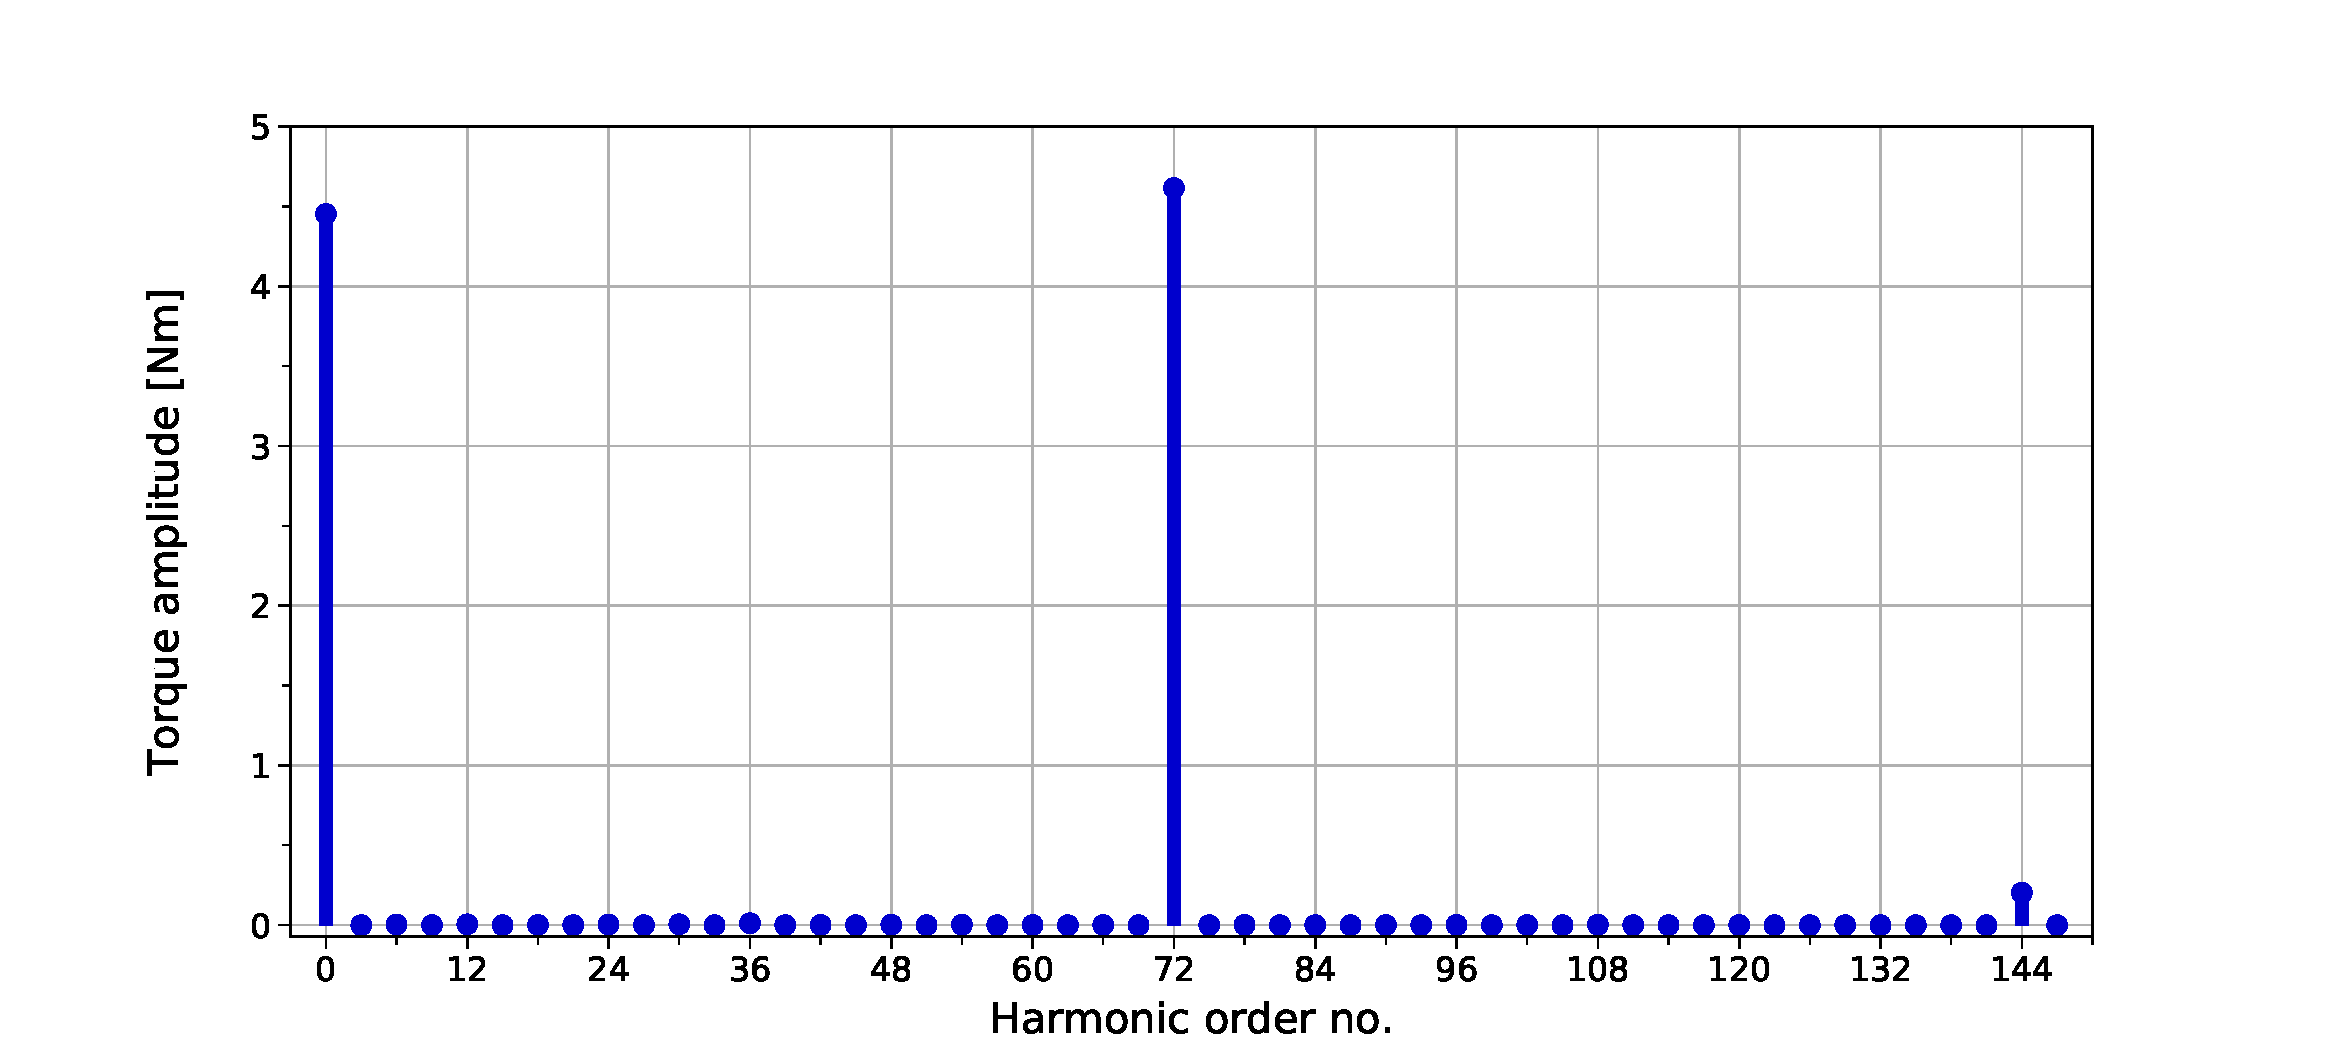
\includegraphics[width=1.0\linewidth]{images/cogging_harmonics.pdf} 
    \caption{Cogging torque harmonics of the $160$-kW motor, when considering the mechanical frequency of the rotor as the fundamental frequency}
    \label{FEM_cogging_harmonics}
\end{figure}

\subsection{Flux harmonics}

Flux density distribution in the airgap and the MMF of the stator windings are seldom ideally sinusoidal. Due to nonsinusoidality, the phase flux linkages contain harmonics of the order of $5,7,11,...$ \cite{TRR_SW:1998}. In rotor reference frame, the corresponding spatial harmonics appear as multiples of sixth-order harmonic components, and can be expressed as \cite{ILC:2004, ILC:2005, ILC:2018}
\begin{equation}
    \psi_{f} = \psi_{d0} + \sum_{j=\text{1}}^{\infty} \psi_{d6j} \, \text{cos}(j6\theta_e)
    \label{flux_harmonics_eq1}
\end{equation}
where $\psi_{d0}$ is the DC term and $\psi_{d6j}$ are the harmonic terms of the d-axis flux linkage, while $\theta_e$ is the electrical angle of the rotor. As before, the flux harmonics could be also considered as a function of the mechanical rotor angle due to relation between mechanical and electrical rotor angles.

Combining \eqref{torque_eq} and \eqref{flux_harmonics_eq1} yields
\begin{equation}
    T_m = T_0 + \sum_{j=\text{1}}^{\infty} T_{6j} \, \text{cos}(j6\theta_e)
    \label{flux_harmonics_eq2}
\end{equation}
where $T_0$ and $T_{6j}$ are the DC component and harmonic torque amplitudes, respectively. Equation \eqref{flux_harmonics_eq2} indicates that produced torque pulsations are periodic in nature. FEM computation done at nominal point with constant speed confirms the periodicity of pulsations and it also shows the sixth harmonic multiples to be especially prominent in Fig. \ref{FEM_flux_harmonics}.

%The periodic tendency can be also observed from finite element method (FEM) computed flux density distribution in Fig. \ref{FEM_flux}. The airgap flux density variation is not smooth enough to be sinusoidal. This density variation induces torque pulsation when the rotor angle changes. 

%Finite element method (FEM) computed flux density distribution of the $160$-kW motor is shown in Fig. \ref{FEM_flux}. The flux harmonics induced by the distribution can be seen in Fig. \ref{FEM_flux_harmonics}. It can be observed that the prominent flux harmonics truly are sixth-multiples of the fundamental frequency. For example, the first harmonic is located at $6 \cdot 155$ Hz $ = 930Hz$.

%\begin{figure}[ht] 
%    \centering
%    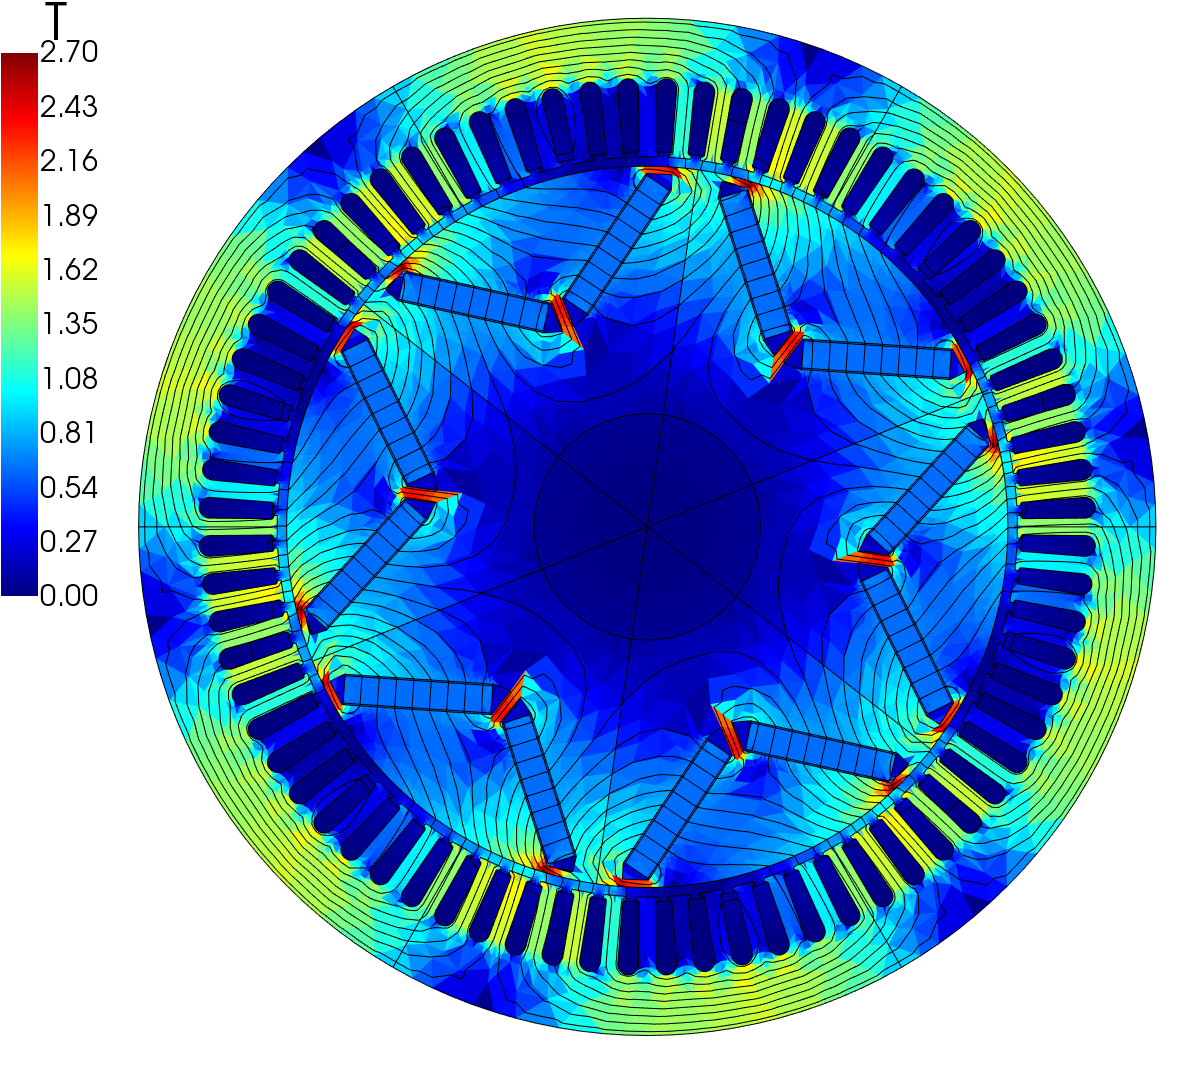
\includegraphics[width=0.6\linewidth]{images/flux_density.png} 
%    \caption{Flux density distribution of the PM motor} 
%    \label{FEM_flux} 
%\end{figure}

\begin{figure}[ht] 
    \centering
    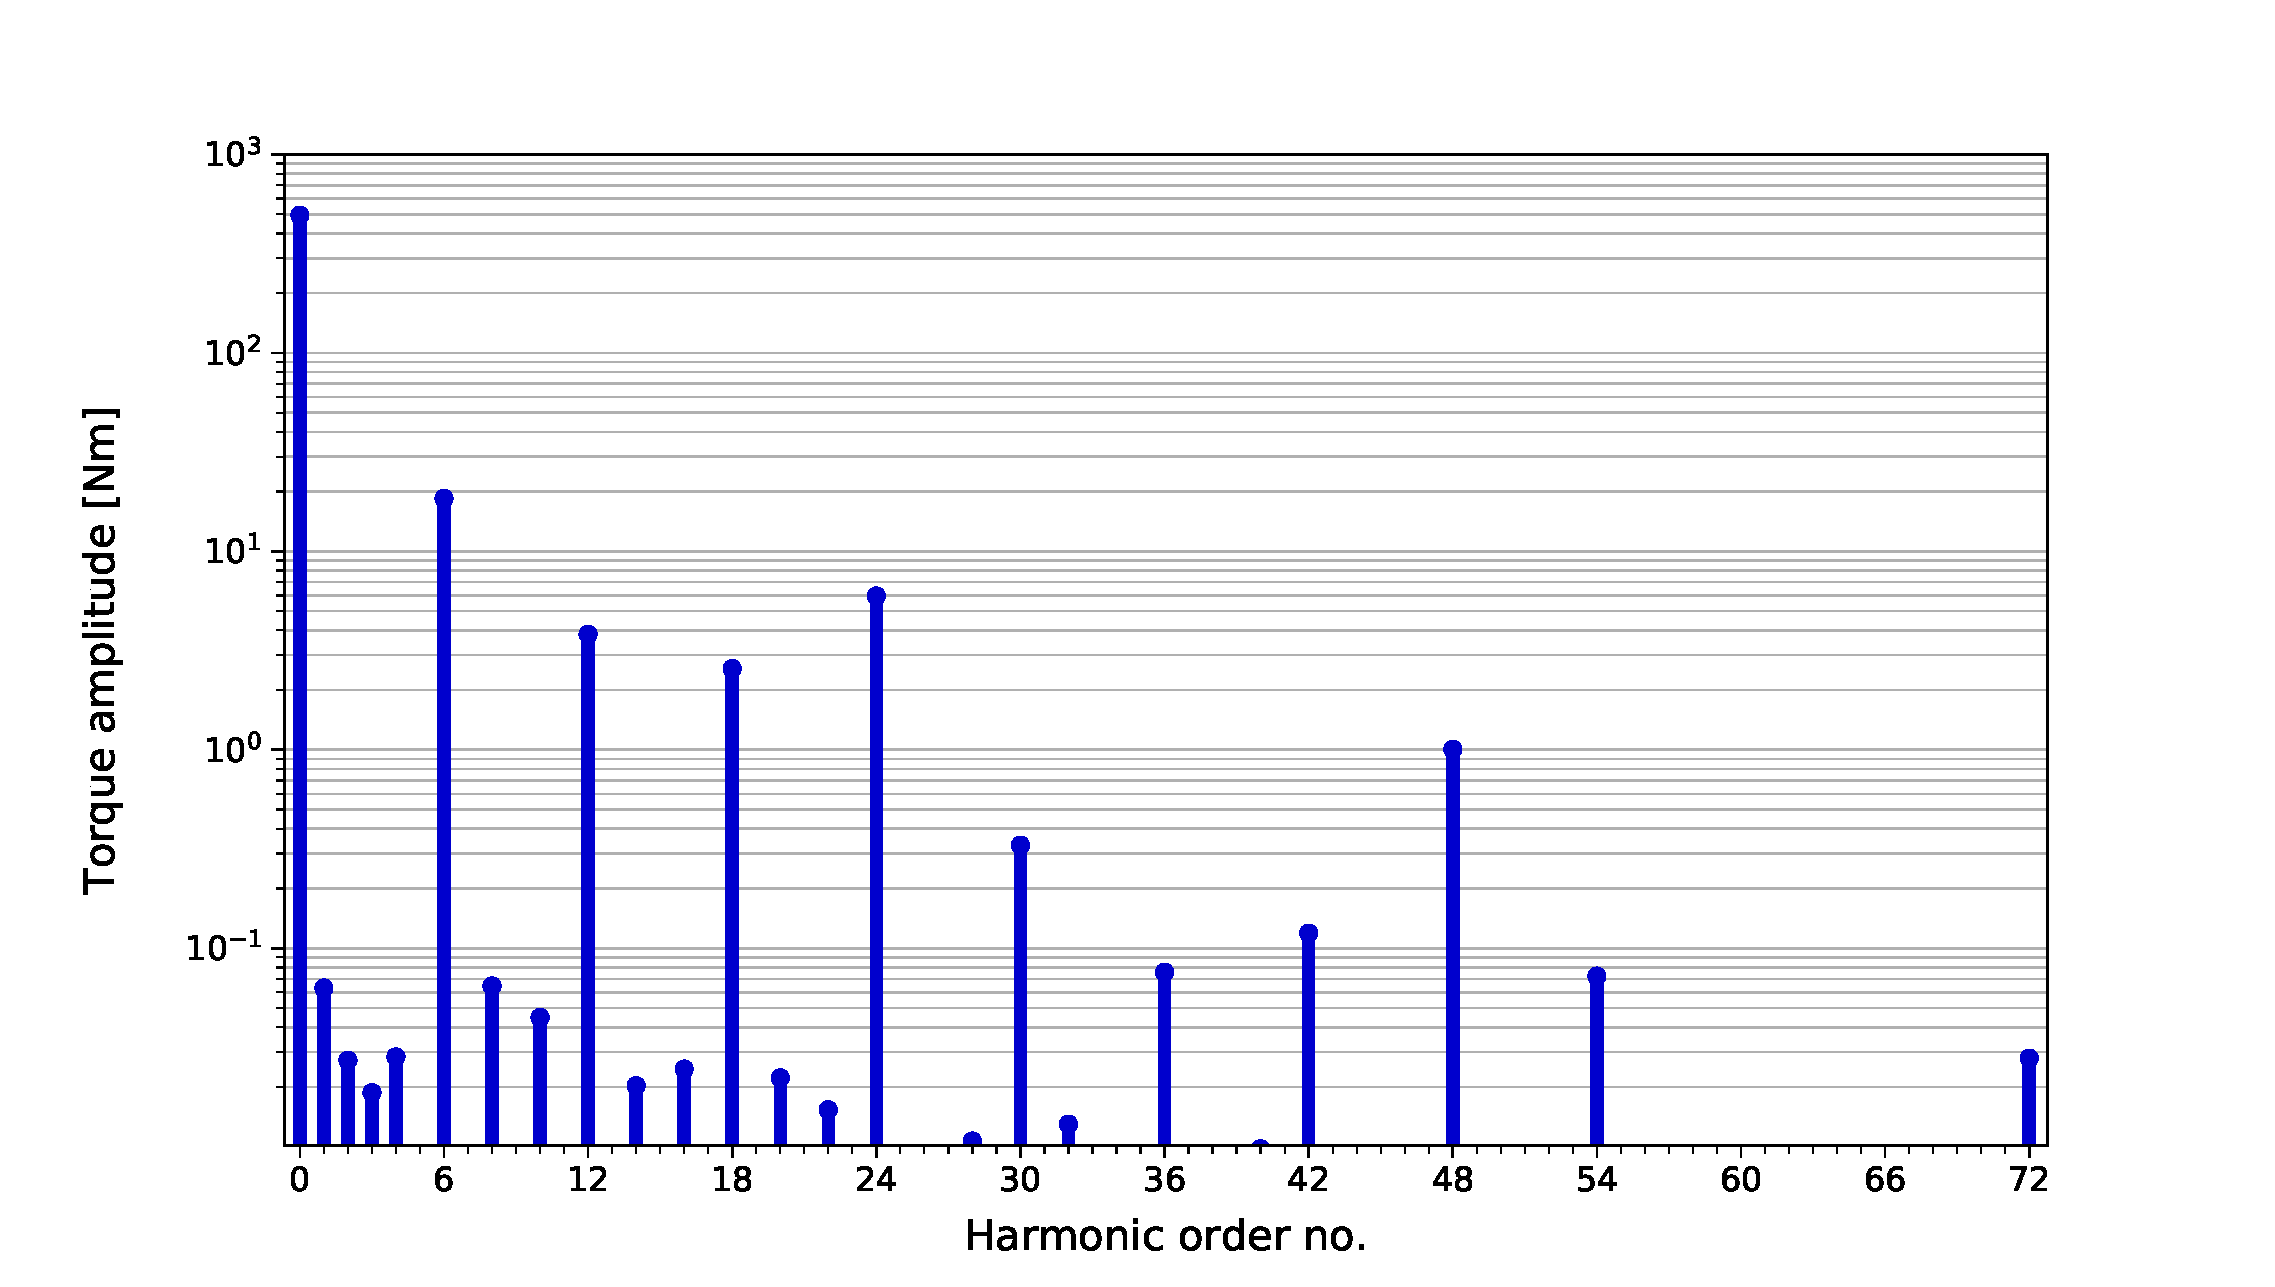
\includegraphics[width=1.0\linewidth]{images/fem-flux-harmonics.pdf} 
    \caption{Torque harmonics of the $160$-kW motor, when considering the supply frequency (155 Hz) as the fundamental frequency}
    \label{FEM_flux_harmonics}
\end{figure}
% Torque harmonics of the $160$-kW motor with respect to the electrical rotor angle, $\theta_e$

It is good to note that Figs. \ref{FEM_flux} and \ref{FEM_flux_harmonics} do not only include the effects of the flux harmonics but also cogging torque, because of overlapping frequencies. When rotor flux is calculated in different rotor angles in time stepping simulation, also cogging torque is inevitably captured. Cogging torque could be subtracted from the result, though this serves no purpose, as the objective is to minimize both disturbances simultaneously.

% ===================================================================================================================
\subsection{Current measurement errors}

Current measurement errors contribute to the torque ripple \cite{current_scaling:1998, ILC:2004, ILC:2005, CTR_SW_ff:2011, ILC:2012, ILC:2018}. The errors can be considered to be the offset and scaling errors \cite{current_scaling:1998, ILC:2004, CTR_SW_ff:2011, ILC:2012}. The stator currents are measured and transduced into voltage signals by current sensors. The voltages are then transformed into digital form by analog-to-digital (A/D) converters \cite{current_scaling:1998, ILC:2005}, so that the control can utilize the measured values. The current measurement errors emerge during this process.

%Practically there is always some amount of current offset. The current scaling errors are also inevitable as A/D conversions has to be made \cite{current_scaling:1998}. The current sensor output must be scaled to match with the A/D converter input, whilst the controller re-scales the converted digital value in order to obtain the actual current value \cite{ILC:2005}.

If there is any unbalance between the phase voltages supplied to the motor, or, if the analog devices include inherent offset, then DC offset current will be introduced. When measuring two phase currents and assuming ideal current control, the current offset related torque error can be described by \cite{current_scaling:1998}
\begin{equation}
    \Delta T_{m1} = k_t \frac{2}{\sqrt{3}}\sqrt{\Delta i_a^2 + \Delta i_a \Delta i_b + \Delta i_b^2} \; \text{cos}(\theta_e + \alpha)
\end{equation}
$$\alpha = \text{tan}^{-1}\left(\frac{\sqrt{3}\Delta i_a}{\Delta i_a + 2 \Delta i_b}\right)$$
where $\Delta i_a$ and $\Delta i_b$ are $a$ and $b$ phase offsets and $\alpha$ represents angular displacement between the phases. The torque error has relation to $\theta_e$, hence DC offsets give rise to torque oscillations at the fundamental frequency \cite{current_scaling:1998, CTR_SW:1998, ILC:2004, ILC:2018}.

A FEM computation with intentionally introduced current offset error was performed. The error was added to single phase current, which was used by control algorithms. The simulation result is shown in Fig. \ref{FEM_current-meas-error}. The introduced error roughly corresponds to 10 A measurement error, which is approximately 3\% of the motor nominal current. With this error, it can be seen that the first harmonic has the greatest amplitude when ignoring the DC component.
\begin{figure}[htb] 
    \centering
    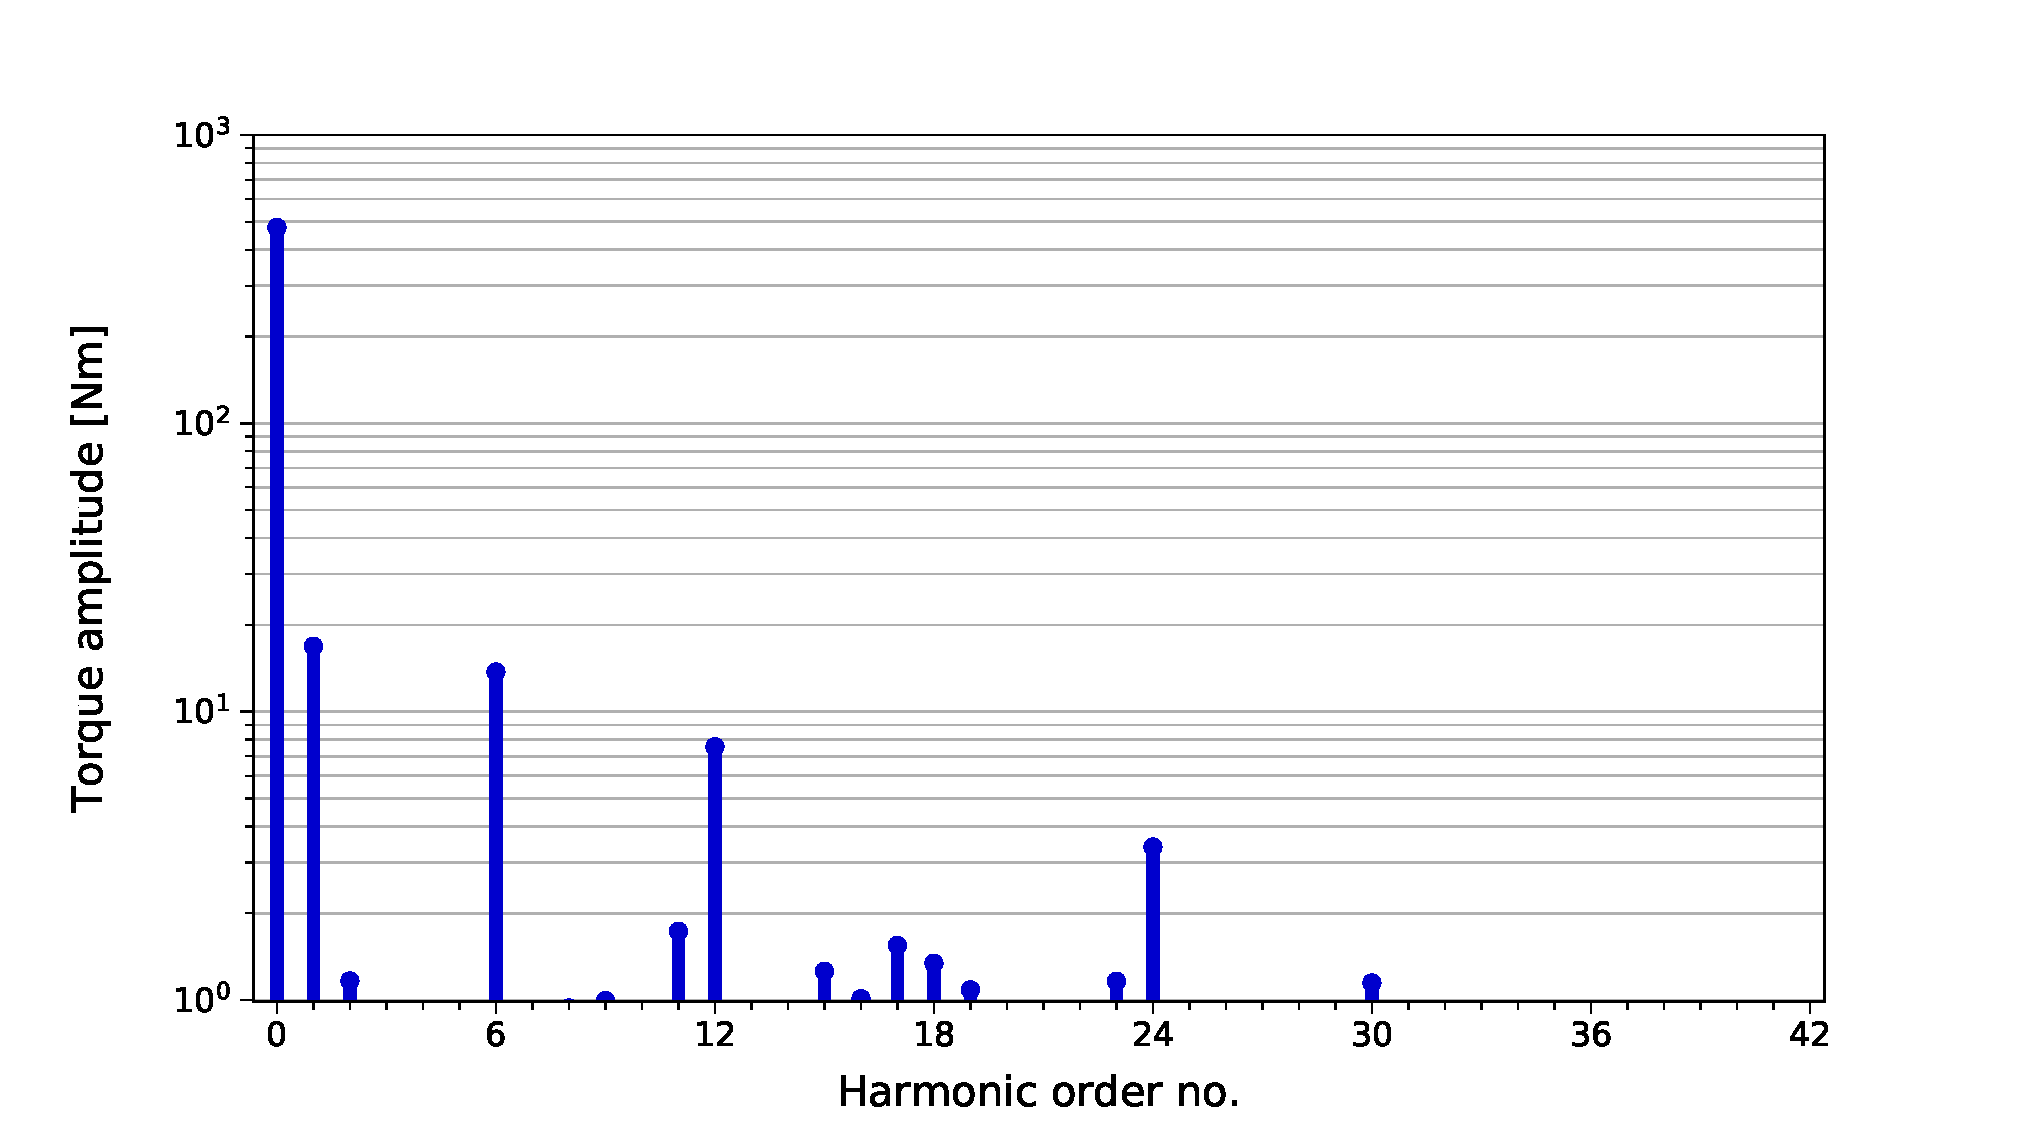
\includegraphics[width=1.0\linewidth]{images/current-measurement-error.pdf} 
    \caption{Torque harmonics of the $160$-kW motor under current measurement error, when considering the supply frequency (155 Hz) as the fundamental frequency}
    \label{FEM_current-meas-error}
\end{figure}

% Torque harmonics of the $160$-kW motor considering the supplied frequency (155 Hz) as fundamental frequency
The measured phase currents must be scaled to fit in the input range of the A/D converter. The A/D converter output is then re-scaled by the current controller, so that real current values can be obtained. Scaling errors are inevitable \cite{current_scaling:1998}. The torque error coming from the scaling errors can be described as \cite{current_scaling:1998, ILC:2005}
\begin{equation}
    \Delta T_{m2} = \left(\frac{K_a - K_b}{K_a K_b}\right) \: \frac{k_t I}{\sqrt{3}} \: \left[\text{cos}\left(2 \theta_e + \frac{\pi}{3}\right)+ \frac{1}{2}\right]
\end{equation}
where $K_a$ and $K_b$ are controller scaling factors for $a$ and $b$ phases and $I$ is the phase current. Since $\theta_e$ is multiplied by two, the scaling errors give rise to torque oscillations at twice the fundamental frequency \cite{current_scaling:1998, ILC:2005, CTR_SW:1998, ILC:2018}.

It can be concluded that torque pulsations resulting from the current measurement errors are periodic with respect to the rotor angle. Therefore, cogging torque, flux harmonics and current measurement errors induce 1st, 2nd, 6th, 12th, etc. torque harmonics and the objective is to suppress these periodic disturbances.

\clearpage
